\chapter{Preliminaries}
\section{Class D Amplifier}
\section{Quadrature amplitude modulation}\label{2_QAM_sec:QAM}
Quadrature amplitude modulation or QAM \cite{nat_skript} is a modulation scheme where an in phase component $I(t)$ and a quadrature component $Q(t)$ are mixed with orthogonal carriers and then added together. The output signal $s(t)$ can be calculated as 
\begin{equation}
    s(t) = I(t) \sin \left ( \omega_0 t\right ) + Q(t)\underbrace{\sin \left ( \omega_0 t + \frac{\pi}{2} \right)}_{\cos{(\omega_0 t)}}
\end{equation}
Through the use of some trigonometric identities this can be simplified to 
\begin{equation}
    s(t) = \sqrt{I^2(t) + Q^2(t)} \sin{\left(\omega_0 t + \arctan{ \left ( \frac{Q(t)}{I(t)} \right )} \right )}
\end{equation}
\section{Piezo-Electric Ultrasoncic Transducer}
Piezo-electric ultrasoncic transducers emit sound by using the reciprocal piezoelectric effect. By applying an electric voltage to piezoelectric material it is deformed and therefore produces ultrasound. Electrically a PUT is best described by using the butterworth van dyke model, which is shown in Figure \ref{2_fig:butt_dyke_model}.
Of which the impedance response looks like \todo{ref}.
\begin{figure}
    \centering
    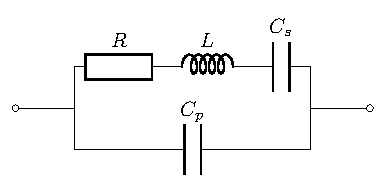
\includegraphics{sections/Van_Dyke_Circuit.pdf}
    \caption{Butterworth van Dyke model}
    \label{2_fig:butt_dyke_model}
\end{figure}
\section{Sigma Delta / Noise Shaping}
Sigma Delta modulators are extremely common analog-digital and digital-analog converters. Their main advantage is their capability to shape noise to be outside of the used bandwidth.
\section{Diffraction from slits}
The principle of Huygens-Fresnel \cite{physik_skript} says that every element on a wave surface can be viewed as a center of a spherical wave and with the variation through time can be calculated. This principle will be used to calculate the diffraction of waves on slits.

In the following it will be discussed how plane wave can be modelled if diffracted by slits if viewed from far enough away.
\subsection{Single-slit diffraction}
All the points inside of the slits are viewed, accordingly to the huygens-fresnel principle, as centers of spherical waves. If we now want to know how the wave behaves at a certain point in space P, with distance r and angle $\phi$, one can superposition all the points inside of the slid
\begin{equation}
    \xi  = \frac{A}{rs}\int_0^s \cos \left ( \omega t - k r + k x \sin\left ( \phi\right )\right) dx.
\end{equation}
Where A is the amplitude of the wave at the slid, $\omega$ is the frequency and k is the wave number given as
\begin{equation}
    k = \frac{\omega}{c}
\end{equation}
This can be simplified to be
\begin{equation}
    \xi = \frac{A}{r}  \underbrace{\frac{\sin \left ( \frac{ks \sin \phi}{2}\right )}{ \frac{ks \sin \phi}{2}}}_{A_s(\phi,k,s)} \cos \left ( \omega t - k r_s\right ).
\end{equation}
The function $A_s(\phi,k,s)$ now shows how the amplitude varies according to the angle, the wave number and the size of the slid. In Figure \todo{ref} it is shown how the amplitude over the angle changes with different frequency while the slit size is hold constant at $s = 0.016m$ for waves with the speed $343m/s$ (speed of sound at 22 degrees Celsius).
\begin{center}
    \begin{minipage}{.49\textwidth}
        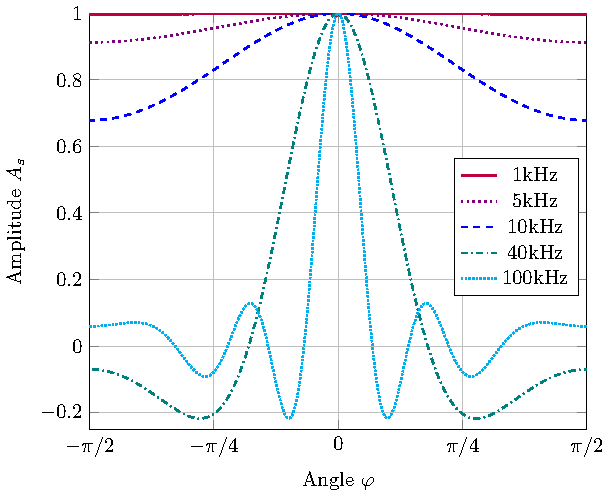
\includegraphics[width=\textwidth]{images/2_Preliminaries/Single_Slid_Frequency.pdf}
    \end{minipage}
    \begin{minipage}{.49\textwidth}
        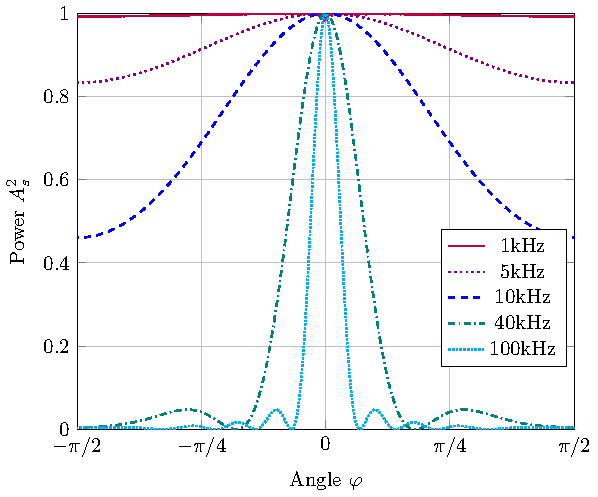
\includegraphics[width=\textwidth]{images/2_Preliminaries/Single_Slid_Frequency_Power.pdf}
    \end{minipage}
\end{center}
\subsection{Diffraction on slits \& Fourier-Transform}\label{2_Acoustics_sec:diffraction_fourier}
One way to calculate the diffraction pattern of a sound wave on slits is to take the Fourier transform of this slits if $f = \frac{x}{\lambda z}$. For example in the case with one slit, which has a size of $a$ and and its middle is at the point $(0,0)$ and edges at $(0,\pm a/2)$ the Fourier transform, which is just a rectangular pulse with the length a, along the z-axis would be equal to
\begin{equation}
    F\left ( \frac{2\pi x}{\lambda z} \right ) = a\frac{\sin{\left(  \frac{\pi x a}{\lambda z} \right )}}{\frac{\pi x a}{\lambda z}} = a\frac{\sin{\left(  \frac{\pi \sin{(\varphi)} a}{\lambda} \right )}}{\frac{\pi \sin{(\varphi)} a}{\lambda}}
\end{equation}
\todo{CHECK}
\subsection{Multiple slits diffraction}
It can be shown that in the case of multiple slits the amplitude of a wave at a certain points given is as
\begin{equation}
    \xi = \frac{A}{r} \underbrace{\frac{\sin \left ( \frac{ks \sin \phi}{2}\right )}{ \frac{ks \sin \phi}{2}} \frac{\sin^2\left( \frac{k d \sin{\varphi}}{2}Z\right )}{\sin^2\left( \frac{k d \sin{\varphi}}{2}\right )}}_{A_{ms}(\phi,k,s)} \cos \left ( \omega t - k r_s\right ).
\end{equation}
Where Z is the number of slits and d is their distance.In Figure \ref{6_fig:multiple_diffraction} an example of a diffraction at multiple slits with different spacing between them is shown.
\begin{figure}
    \centering
    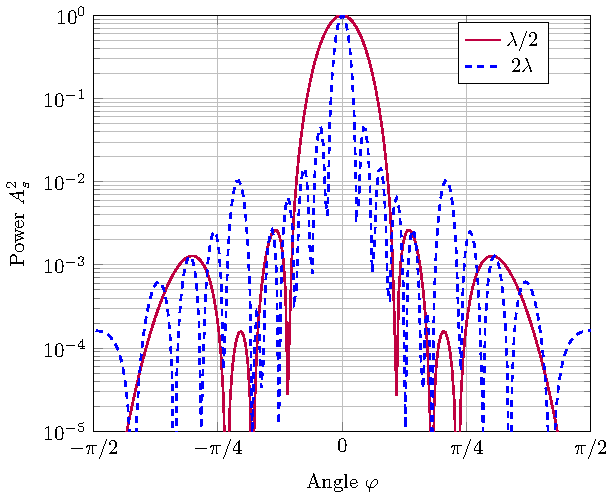
\includegraphics[width=0.7\textwidth]{images/2_Preliminaries/Multiple_Slid_Count.pdf}
    \caption{Diffraction on multiple slits}
    \label{6_fig:multiple_diffraction}
\end{figure}
\section{Acoustics}
\subsection{Basics}
A sound wave is a disturbance propagated through  a material (mostly air in acoustics) which causes a variation in pressure.
This disturbance in the ambient pressure is the sound pressure and is proportional to the inverse of the squared distance to the source.\cite{BERANEK20121}
\begin{equation}\label{2_Acoustics_eq:Pressure_sphere}
    p(r) \propto \frac{1}{r^2}.
\end{equation}
To get a better feeling for sound pressure in Table \ref{2_Acoustics_tab:Sound_pressure_level} are some examples of different sound sources, distances and their sound pressure. \cite{rossing1990science}
\begin{center}
\begin{table}[]
    \centering
    \begin{tabular}{| c | c | c | c |} 
     \hline 
     Sound source & Distance & Sound Pressure [Pa] & SPL [dB ref. 20$\mu$Pa] \\ 
     \hline
     Jet takeoff & 60m & 20 & 120 \\  
     Loud shouting & 1.5m & 2 & 100 \\
     Busy street & - & 0.2 & 80 \\
     Normal conversation & 1m & 0.02 & 60 \\
     Hearing threshold & - & 0.00002 & 0 \\
      \hline
    \end{tabular}
    \caption{Sound sources and their respective sound pressure (level)}
    \label{2_Acoustics_tab:Sound_pressure_level}
\end{table}
\end{center}
Additionally the sound pressure level (SPL) $L_p$ is displayed. It is the logarithmic measure of sound pressure $p$ relative to a reference value $p_0$.
\begin{equation}
    L_p 
    =
    20 \log_{10} \left ( \frac{p}{p_0} \right ) [dB].
\end{equation}
Mostly this reference value is picked to be $20 \mu Pa$ which is the hearing threshold for humans. \cite{rossing1990science}
\subsection{Sound power}
The sound power is the total sound energy emitted by a loudspeaker. Often instead of the sound power the sound power level is used. This sound power level $L_W$ is the logarithmic measure of sound power $P$ relative to a reference power $P_0$
\begin{equation}
    L_W = 10\log_{10} \left (  \frac{P}{P_0} \right ) [dB].
\end{equation}
The reference power is often chosen to be $1pW$. \cite{rossing1990science}
\subsection{Directivity}
In this application specially the directivity of a sound source is of high importance, due to the goal of creating a highly directional beam. 
The directivity of s a sound source is expressed as its directivity factor $Q_D$. It is definded as \cite{DirectivityIndices}
\begin{equation}\label{2_Acoustics_eq:Directivity}
    Q_D = \frac{|p_{axis}|^2}{\rho_0 c}\frac{4 \pi r^2}{W} = \frac{4 \pi p_{rms}^2}{2\pi\int_0^{\pi}p^2_{rms}(\theta)\sin{\theta}d\theta} 
\end{equation}
\subsection{Sound power level vs. Sound pressure level}
The sound pressure level at any point can be calculated through the distance to the source $r$, the sound power level of the source and the directivity and can be calculated, according to \cite{Relationship_Sound_pressure}, as
\begin{equation}\label{2_Acoustics_eq:SPLvSPL}
    L_p = L_W + 10\log_{10}\left( \frac{Q_D}{4 \pi r^2} + \frac{4}{R_c} \right ).
\end{equation}
Where $R_c$ is the room constant given as
\begin{equation}
    R_c = \frac{S\alpha_{av}}{1 - \alpha_{av}} [m^3].
\end{equation}
Here $S$ stands for the volume  and $\alpha_{av}$ is the average absorption coefficient of the room.  If the room is large enough ($S >> 1$) then $R_c >> 1$ follows which means Equation \ref{2_Acoustics_eq:SPLvSPL} can be simplified to
\begin{equation}
     L_p 
     = 
     L_W + 10\log_{10}\left( \frac{Q_D}{4 \pi r^2} \right ) 
     =
     L_W + 10\left ( \log_{10}(Q_D) - \log_{10}(r^2) - \underbrace{\log_{10}(4\pi)}_{\approx 1.1}  \right ). 
\end{equation}